%%%%%%%%%%%%%%%%%%%%%%%%%%%%%%%%%% Niels %%%%%%%%%%%%%%%%%%%%%%%%%%%%%
%%%%%%%%%%%%%%%%%
\section{Communication}

\begin{frame}{Communication}{}
  \begin{figure}
  	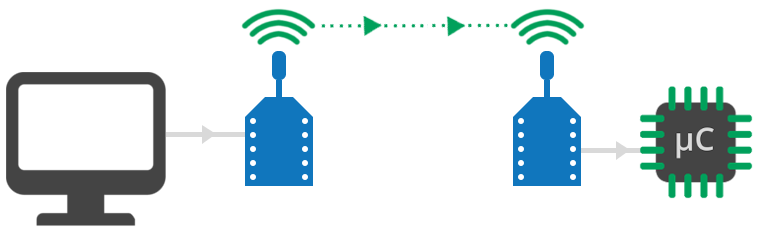
\includegraphics[scale = .45]{Pictures/xbeeSerialConnection.png}
  \end{figure}
\end{frame}
%%%%%%%%%%%%%%%%%

%%%%%%%%%%%%%%%%
\subsection{Filtering}

\begin{frame}{Communication}{Filtering}
  \begin{itemize}
    \item Spikes from GoT system
    \item Removing unlikely data points prior transmission
  \end{itemize}
  
  \begin{figure}
  	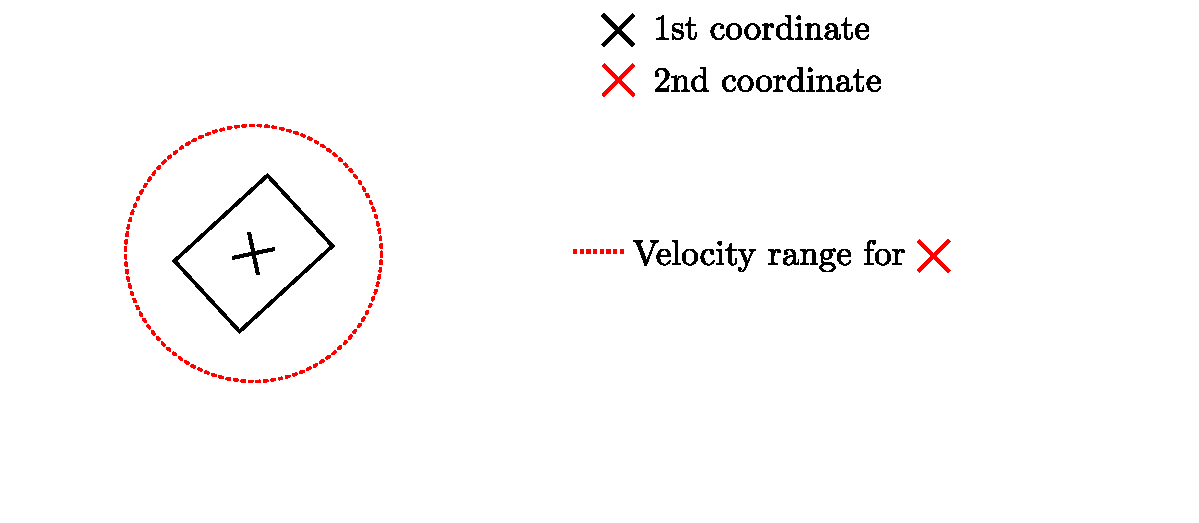
\includegraphics[scale = .5]{Pictures/comFilter1.pdf}
  \end{figure}
  
\end{frame}
\begin{frame}{Communication}{Filtering}
  \begin{itemize}
    \item Spikes from GoT system
    \item Removing unlikely data points prior transmission
  \end{itemize}
  
  \begin{figure}
  	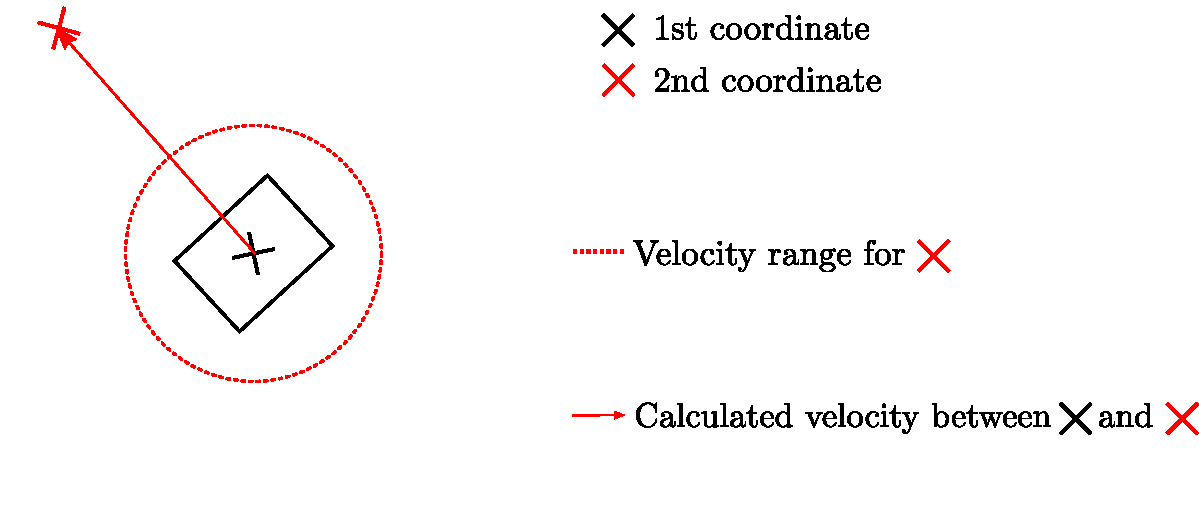
\includegraphics[scale = .5]{Pictures/comFilter2.pdf}
  \end{figure}
  
\end{frame}
\begin{frame}{Communication}{Filtering}
  \begin{itemize}
    \item Spikes from GoT system
    \item Removing unlikely data points prior transmission
  \end{itemize}
  
  \begin{figure}
  	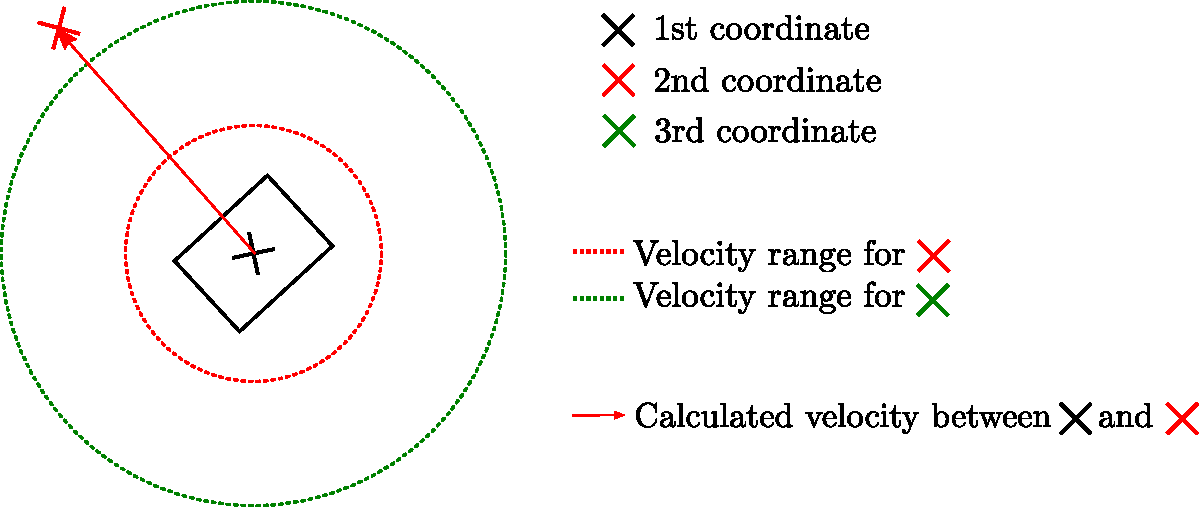
\includegraphics[scale = .5]{Pictures/comFilter3.pdf}
  \end{figure}
  
\end{frame}
\begin{frame}{Communication}{Filtering}
  \begin{itemize}
    \item Spikes from GoT system
    \item Removing unlikely data points prior transmission
  \end{itemize}
  
  \begin{figure}
  	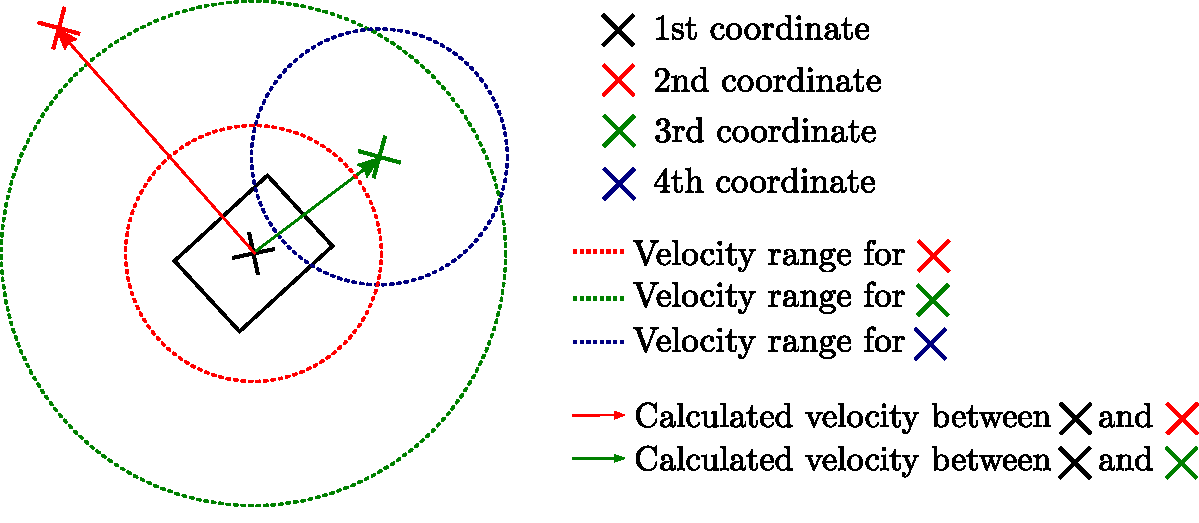
\includegraphics[scale = .5]{Pictures/comFilter4.pdf}
  \end{figure}
  
\end{frame}
\begin{frame}{Communication}{Filtering}
  \begin{itemize}
    \item Spikes from GoT system
    \item Removing unlikely data points prior transmission
  \end{itemize}
  
  \begin{figure}
  	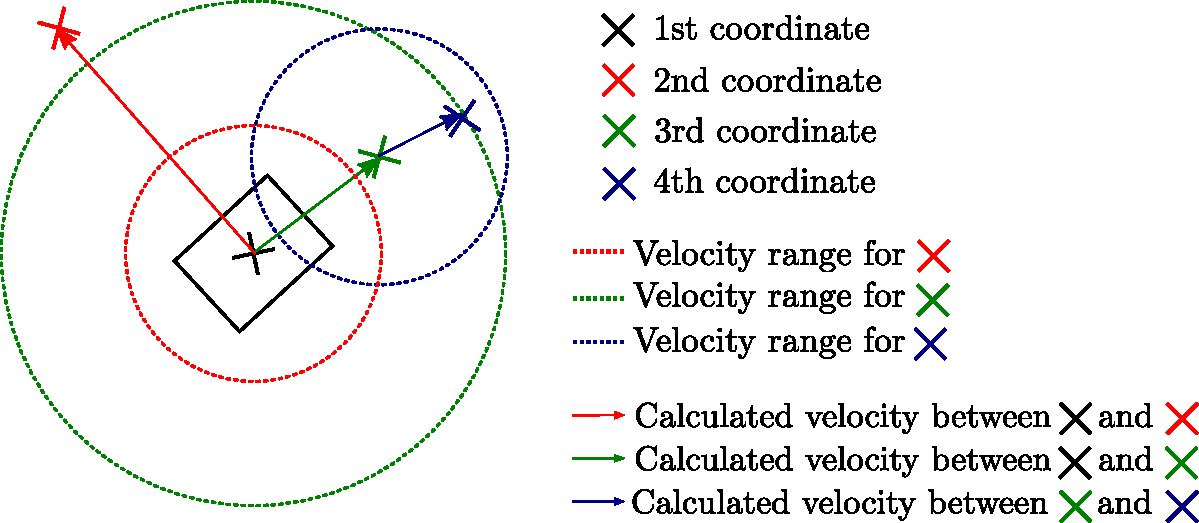
\includegraphics[scale = .5]{Pictures/comFilter5.pdf}
  \end{figure}
\end{frame}
%%%%%%%%%%%%%%%%

%%%%%%%%%%%%%%%%
\subsection{Basis}
\begin{frame}{Communication}{Basis}

  \begin{itemize}
    \item XBee modules
  \end{itemize}
  
  \begin{figure}
    	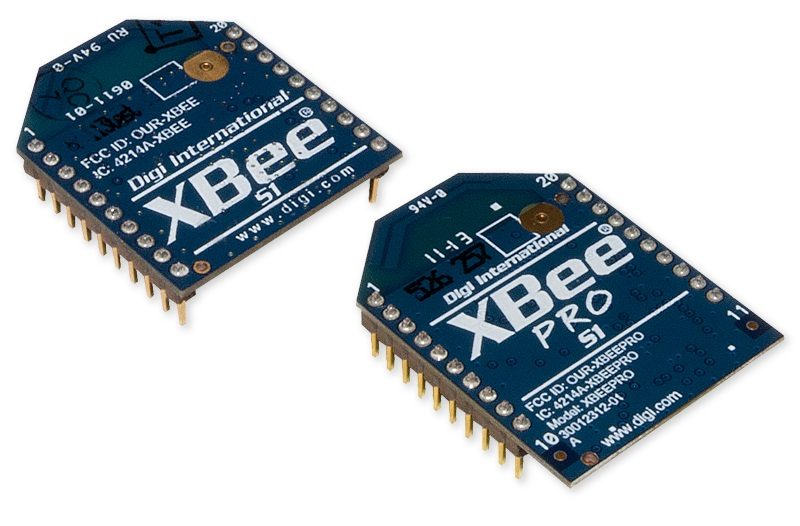
\includegraphics[scale = .1]{Pictures/Xbee.jpg}
  \end{figure}
  \vspace{-.2cm}
  \begin{itemize}
    \item Data path:\\GoT computer $\rightarrow$ XBee $\rightarrow$ XBee $\rightarrow$ microcontroller
    \item No re-transmissions since data is used for feedback 
    \item Connection less protocol
    \item Focus on transport layer for reliable data reception
  \end{itemize}
  
\end{frame}
%%%%%%%%%%%%%%%%

%%%%%%%%%%%%%%%%
\subsection{Package Transport}
  \begin{frame}{Communication}{Package Transport}
  
  \begin{itemize}
    \item The structure of a package
  \end{itemize}
  \begin{table}[H]\centering\vspace{-.2cm}
	\begin{tabular}{|l|l|l|c|l|c|l|l|}
	  \cline{1-3}\cline{5-5}\cline{7-8}%----------------------------------    ----------------------    -----------------------------------------------------
		\footnotesize Start byte & \footnotesize ID & \footnotesize Length &    & \footnotesize Data &    & \footnotesize Checksum & \footnotesize End byte \\
		\cline{1-3}\cline{5-5}\cline{7-8}%----------------------------------    ----------------------    -----------------------------------------------------
	\end{tabular}
  \end{table}
  \vspace{-.25cm}
  \hspace{1.8cm} Header \hspace{1.4cm} Body \hspace{1.8cm} Tail
  \vspace{.25cm}
  
  \begin{itemize}
      \item ID of receiver and length of package are constant in this case
      \item Checksum can be larger/more effective with larger packets
      \item Packages may be lost
      \item Risk of fallacious packages being accepted is very slim
  \end{itemize}
 
\end{frame}
%%%%%%%%%%%%%%%%



%%%%%%%%%%%%%%%%%
\section{Digital Filter}

\begin{frame}{Digital Filter}{}
\vspace{-4cm}
  \begin{figure}
  \hspace{-.8cm}
    	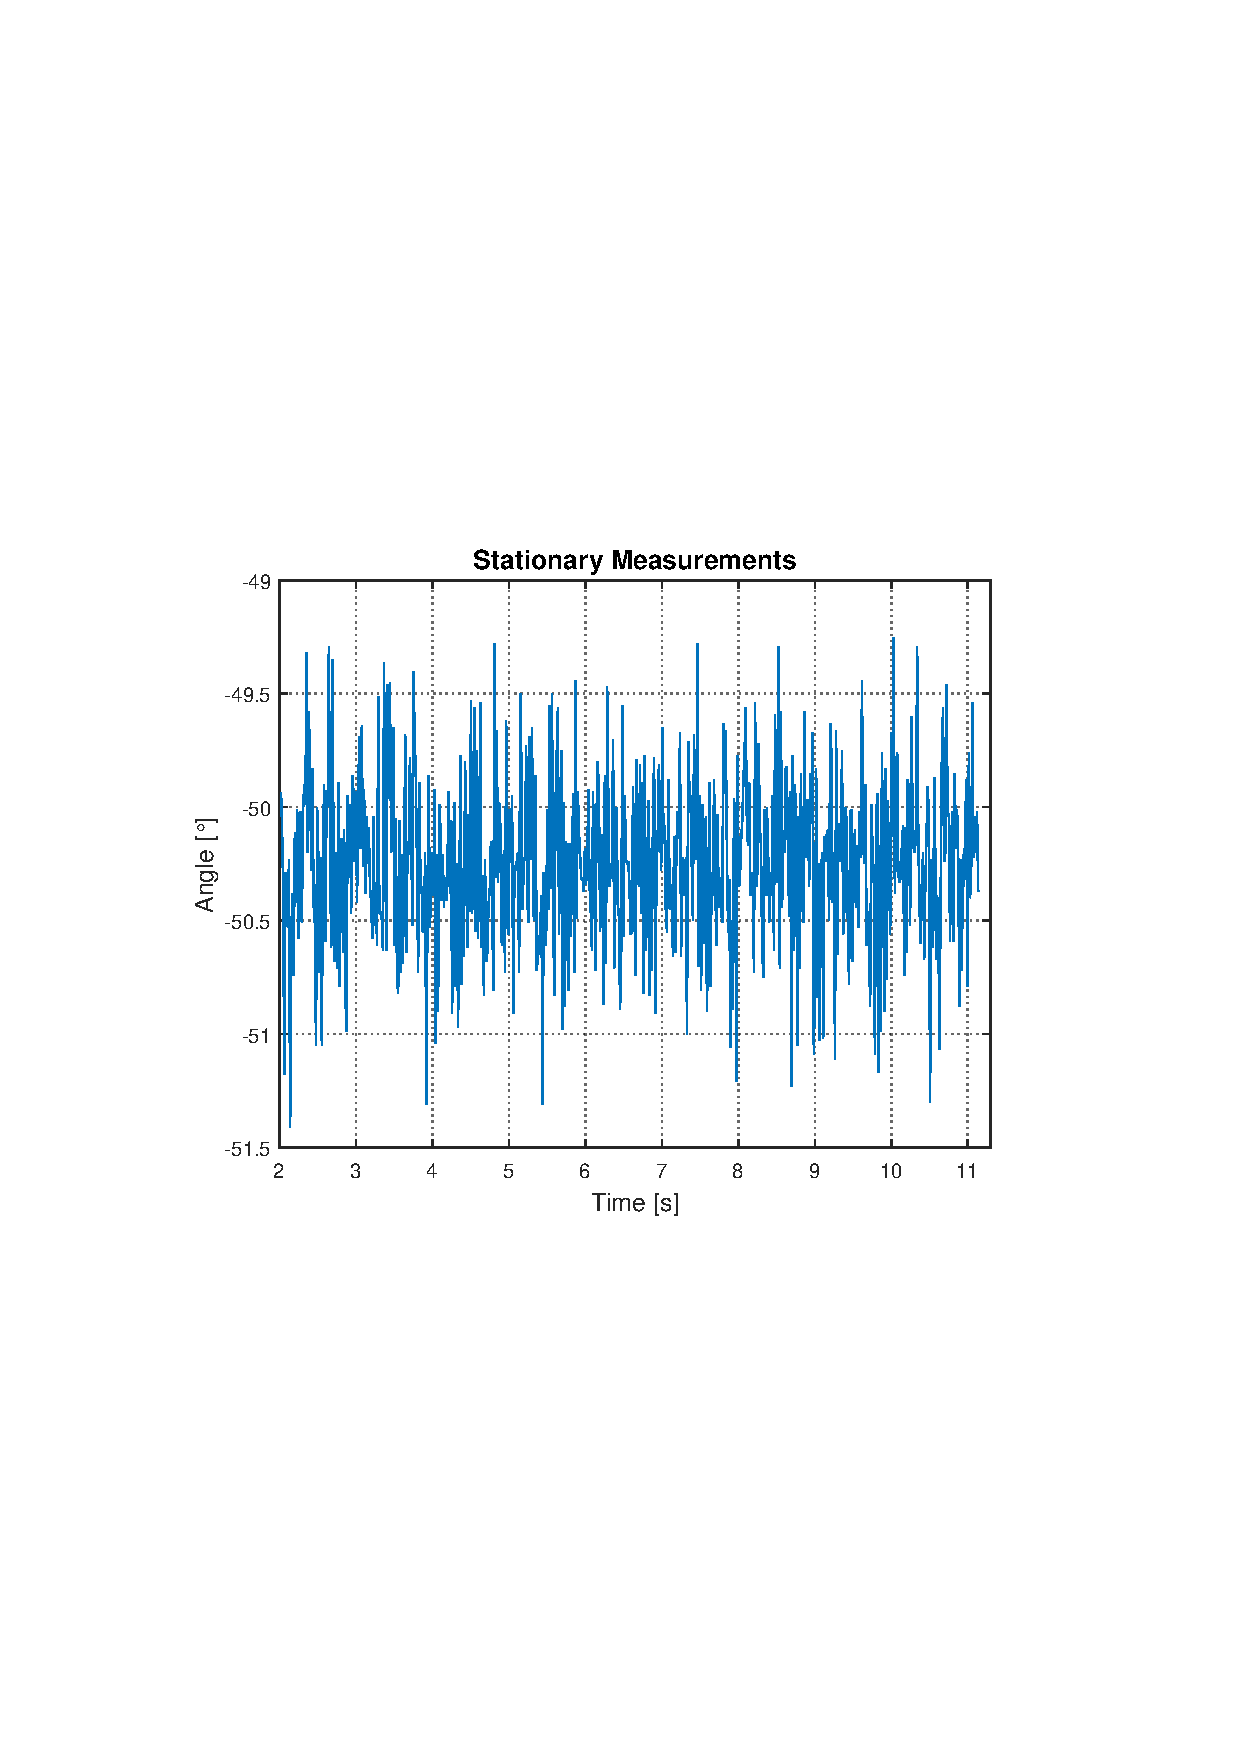
\includegraphics[scale = .5]{Pictures/StationaryMeasurements.pdf}
  \end{figure}
\end{frame}
%%%%%%%%%%%%%%%%%

%%%%%%%%%%%%%%%%
\subsection{Magnitude of Frequencies}
\begin{frame}{Digital Filter}{Magnitude of Frequencies}
\vspace{-4cm}
  \begin{figure}
  \hspace{-.8cm}
    	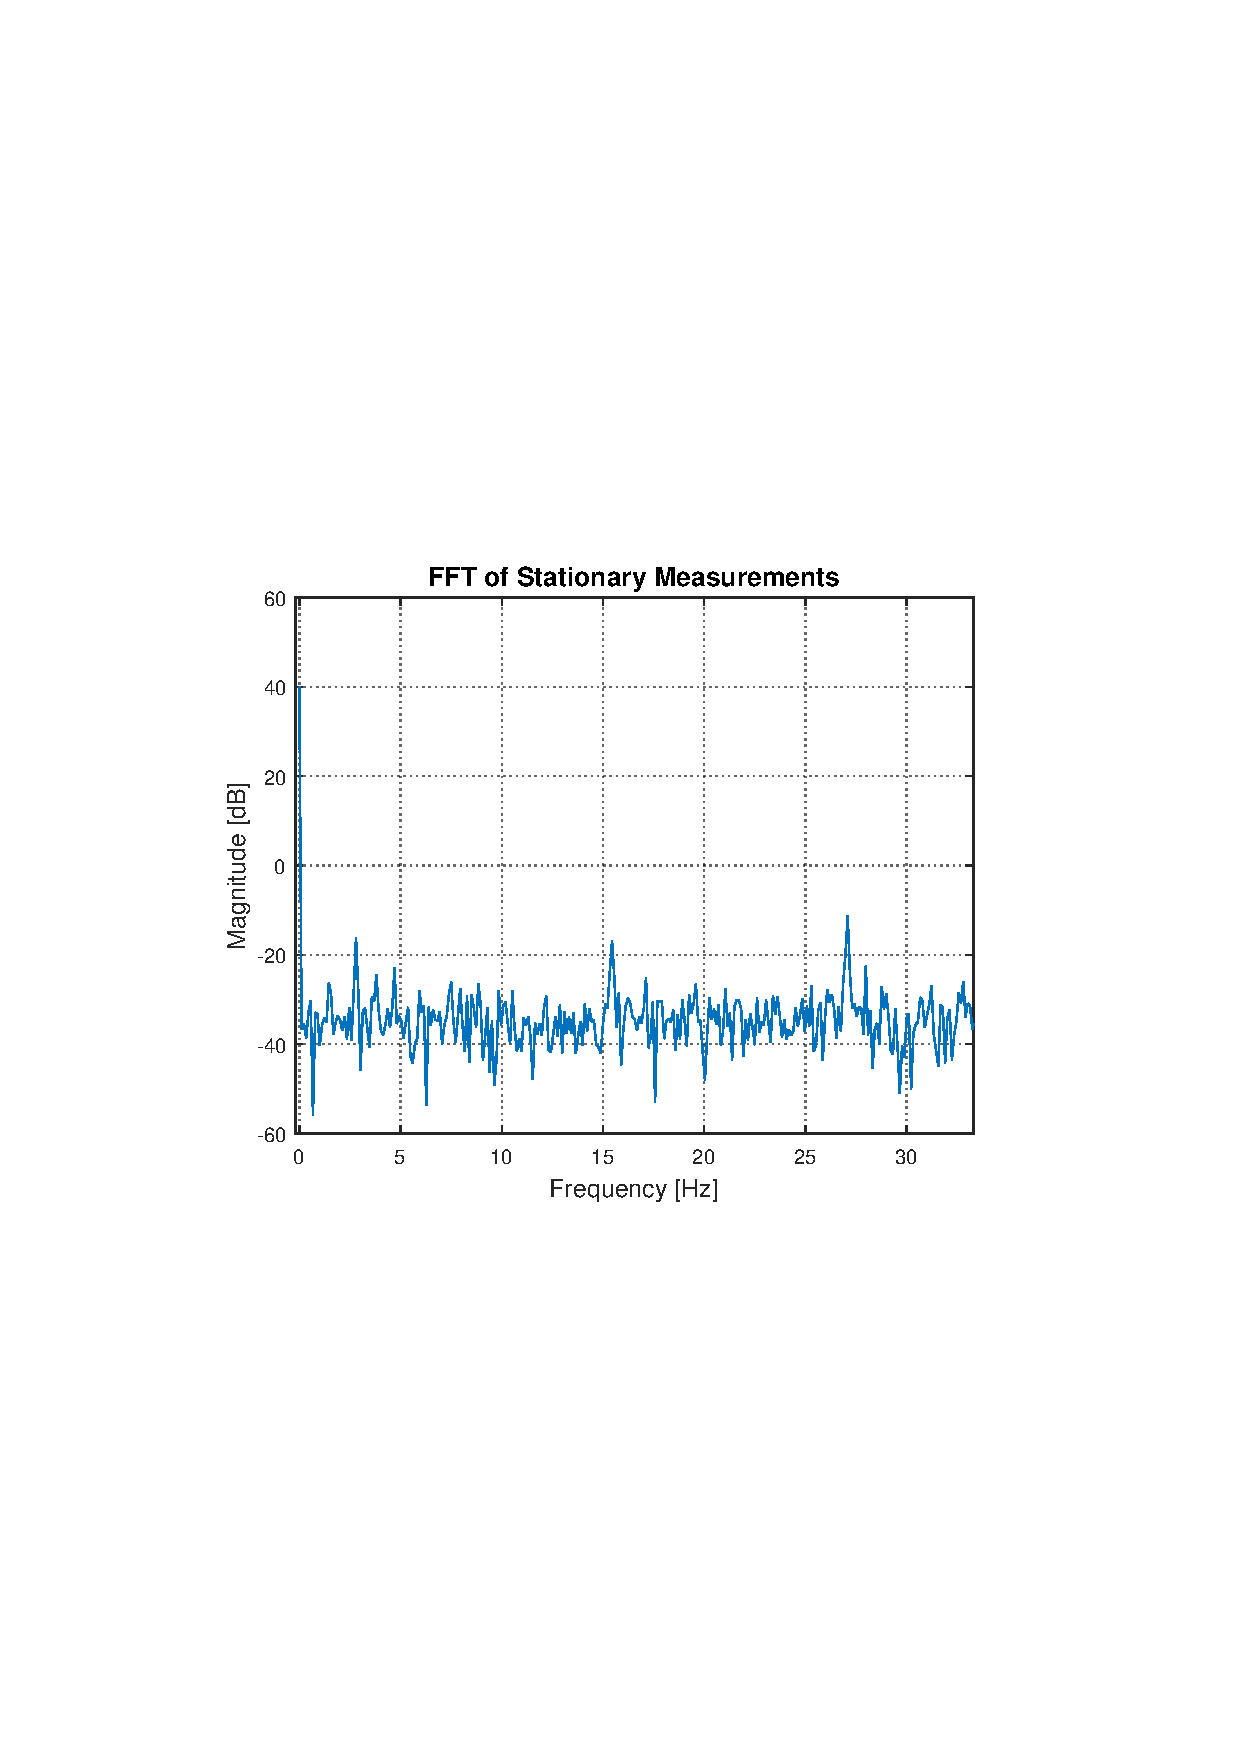
\includegraphics[scale = .5]{Pictures/FFTofStationaryMeasurements.pdf}
  \end{figure}
\end{frame}
%%%%%%%%%%%%%%%%

%%%%%%%%%%%%%%%%
\subsection{Filter Specifications}
\begin{frame}{Digital Filter}{Filter Specifications}
  \begin{itemize}
      \item Inner loop of steering plant
  \end{itemize}
  \vspace{-.4cm}
  \begin{flalign}
      \text{H(s)} = \frac{\text{K}}{(0.03\text{s}+1)\text{s}} \nonumber
  \end{flalign}
  \begin{figure}
    \vspace{-.8cm}\hspace{.4cm}
    
\includegraphics[scale = .4]{Pictures/steeringEqFilter.pdf}
  \end{figure}
  \vspace{-.5cm}\hspace{2cm}
  Highest placed pole is at 33,33 rad$\cdot\text{s}^{-1}$\\
  \hspace{2cm} One decade above: 333,33 rad$\cdot\text{s}^{-1}\ =$ 53 Hz
  \vspace{.1cm}
  \begin{itemize}
    \item Sample rate by Nyquist
  \end{itemize}
  \vspace{-.3cm}
  \begin{flalign}
    \Omega_s \geq 2 \cdot 53 \text{ Hz} \Rightarrow  \Omega_s \geq 106 \text{ Hz} \nonumber
  \end{flalign}
  \vspace{-.6cm}
  \begin{itemize}
    \item Max magnetometer sample rate is 75 Hz
    \item Filter specifications chosen iteratively
    \item Choice of 66.66 Hz will affect phase
    \item Chosen filter type: Low pass Butterworth
  \end{itemize}
  
\end{frame}
%%%%%%%%%%%%%%%%

%%%%%%%%%%%%%%%%
\subsection{Discrete Time}
\begin{frame}{Digital Filter}{Discrete Time}
  \vspace{-4cm}
    \begin{figure}
    \hspace{-.8cm}
      	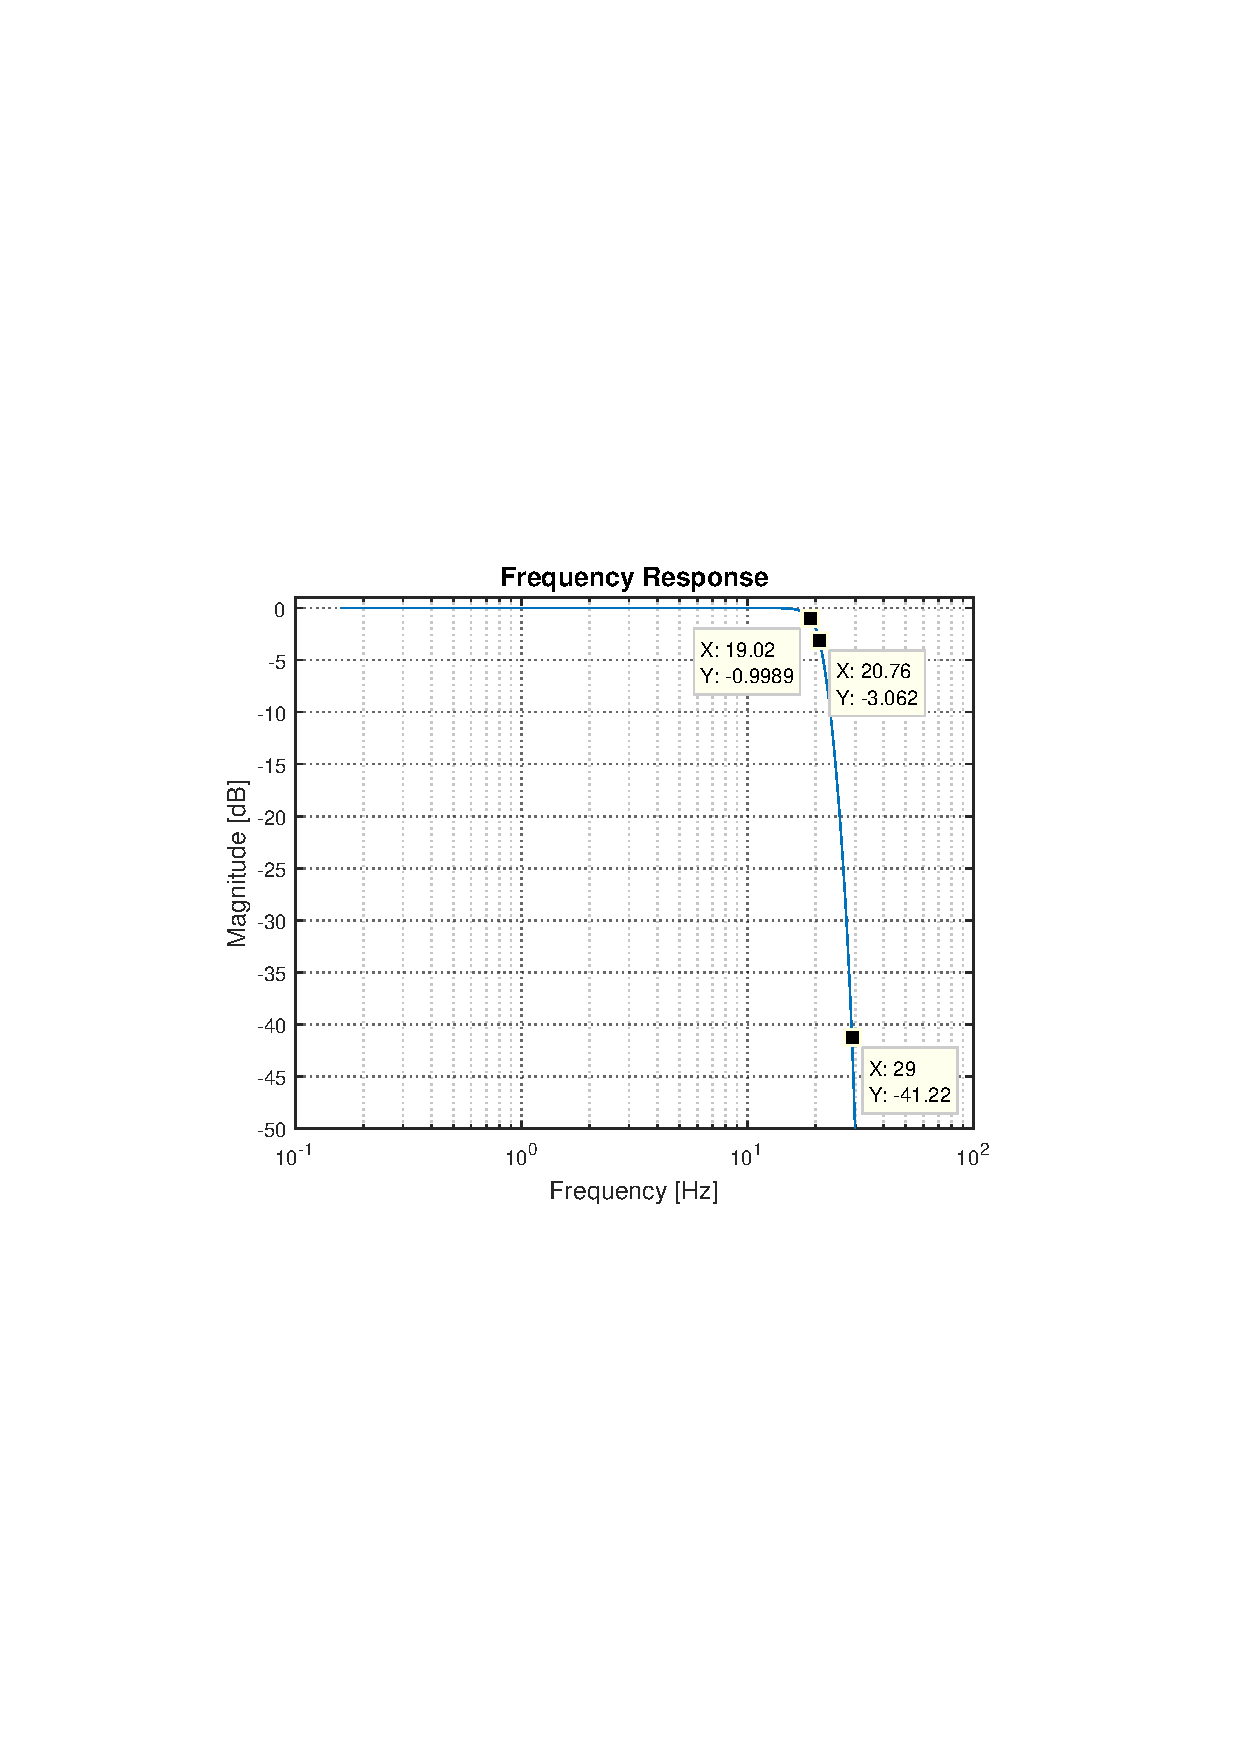
\includegraphics[scale = .5]{Pictures/DiscreteFrequencyResponse.pdf}
    \end{figure}
\end{frame}
%%%%%%%%%%%%%%%%

%%%%%%%%%%%%%%%%
\subsection{Result and Conclusions}
\begin{frame}{Digital Filter}{Result and Conclusions}
\vspace{-4cm}
  \begin{figure}
  \hspace{-.8cm}
    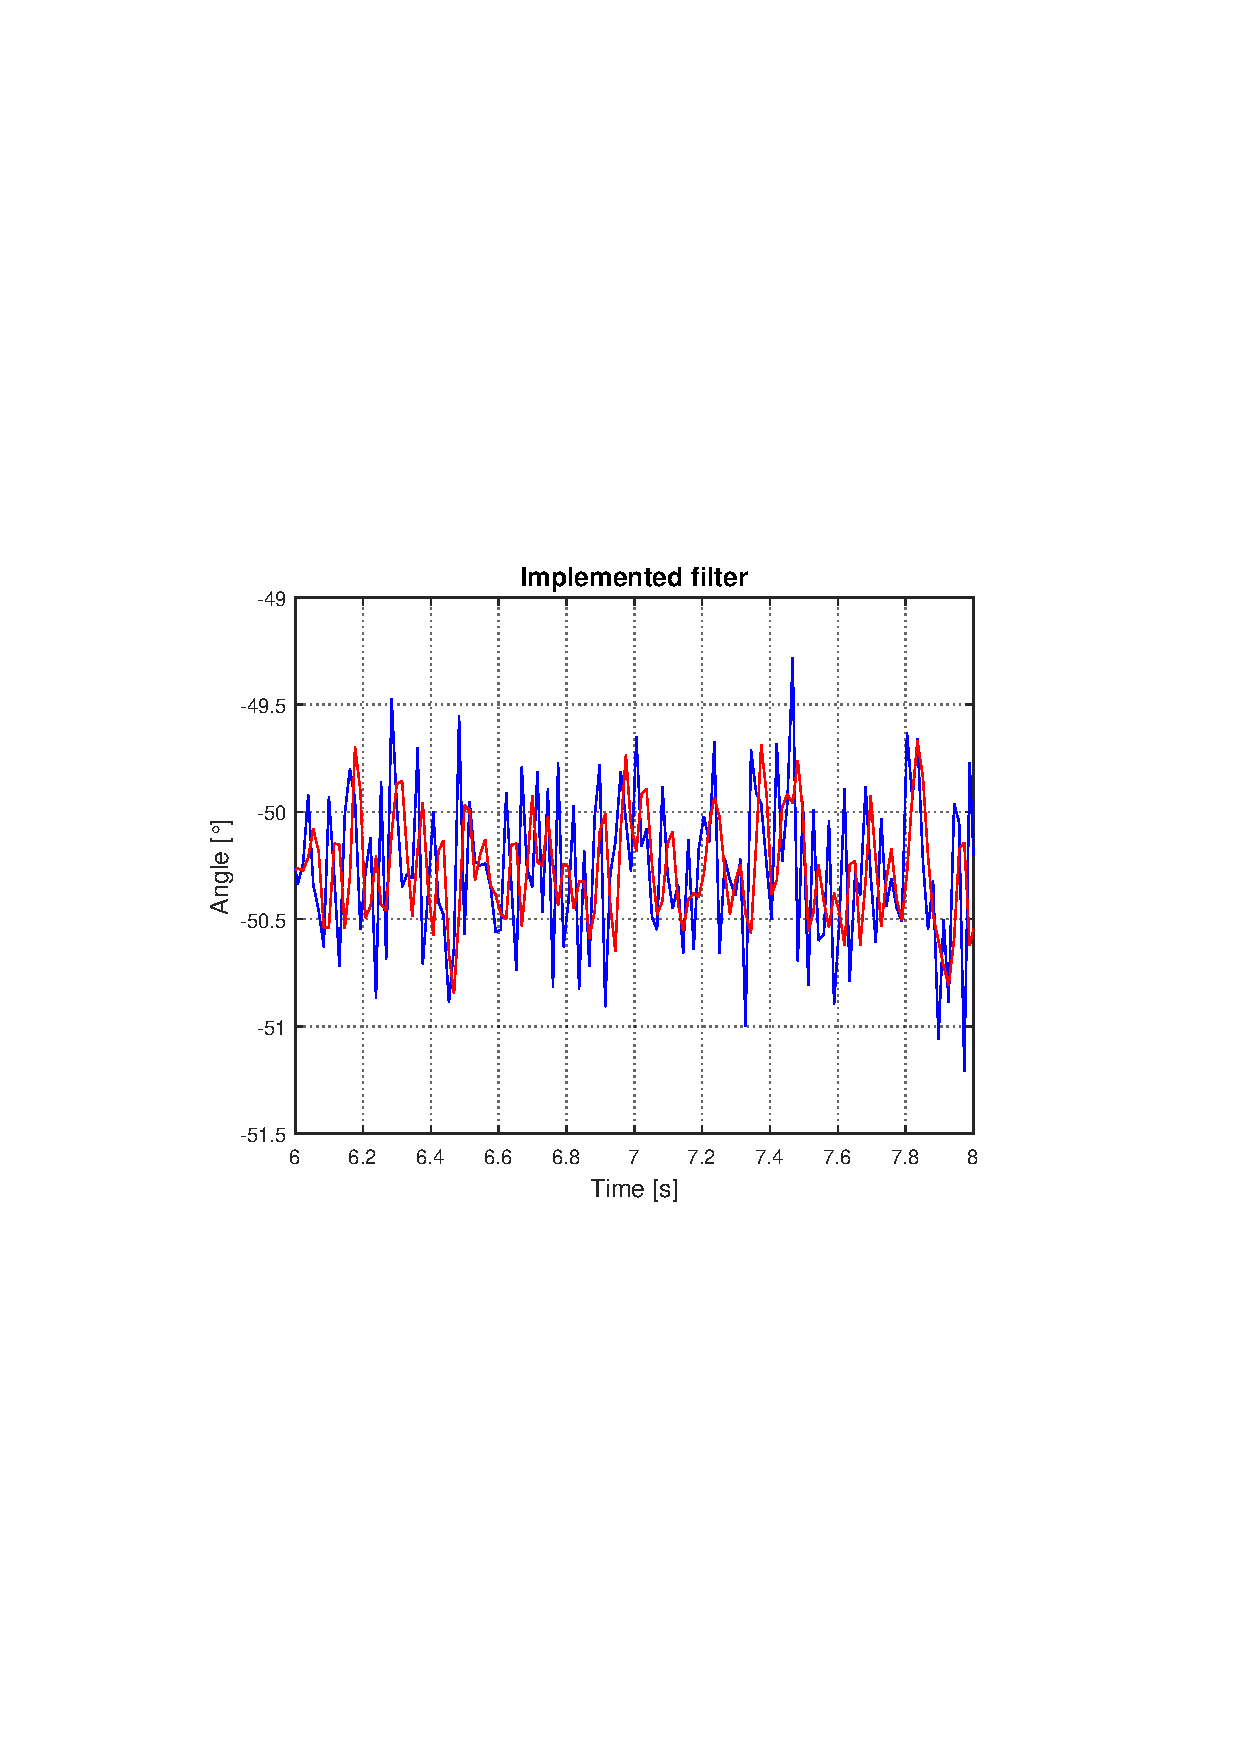
\includegraphics[scale = .5]{Pictures/ImplementedFilter.pdf}
  \end{figure}
\end{frame}

\begin{frame}{Digital Filter}{Result and Conclusions}
\vspace{-4cm}
  \begin{figure}
  \hspace{-.8cm}
    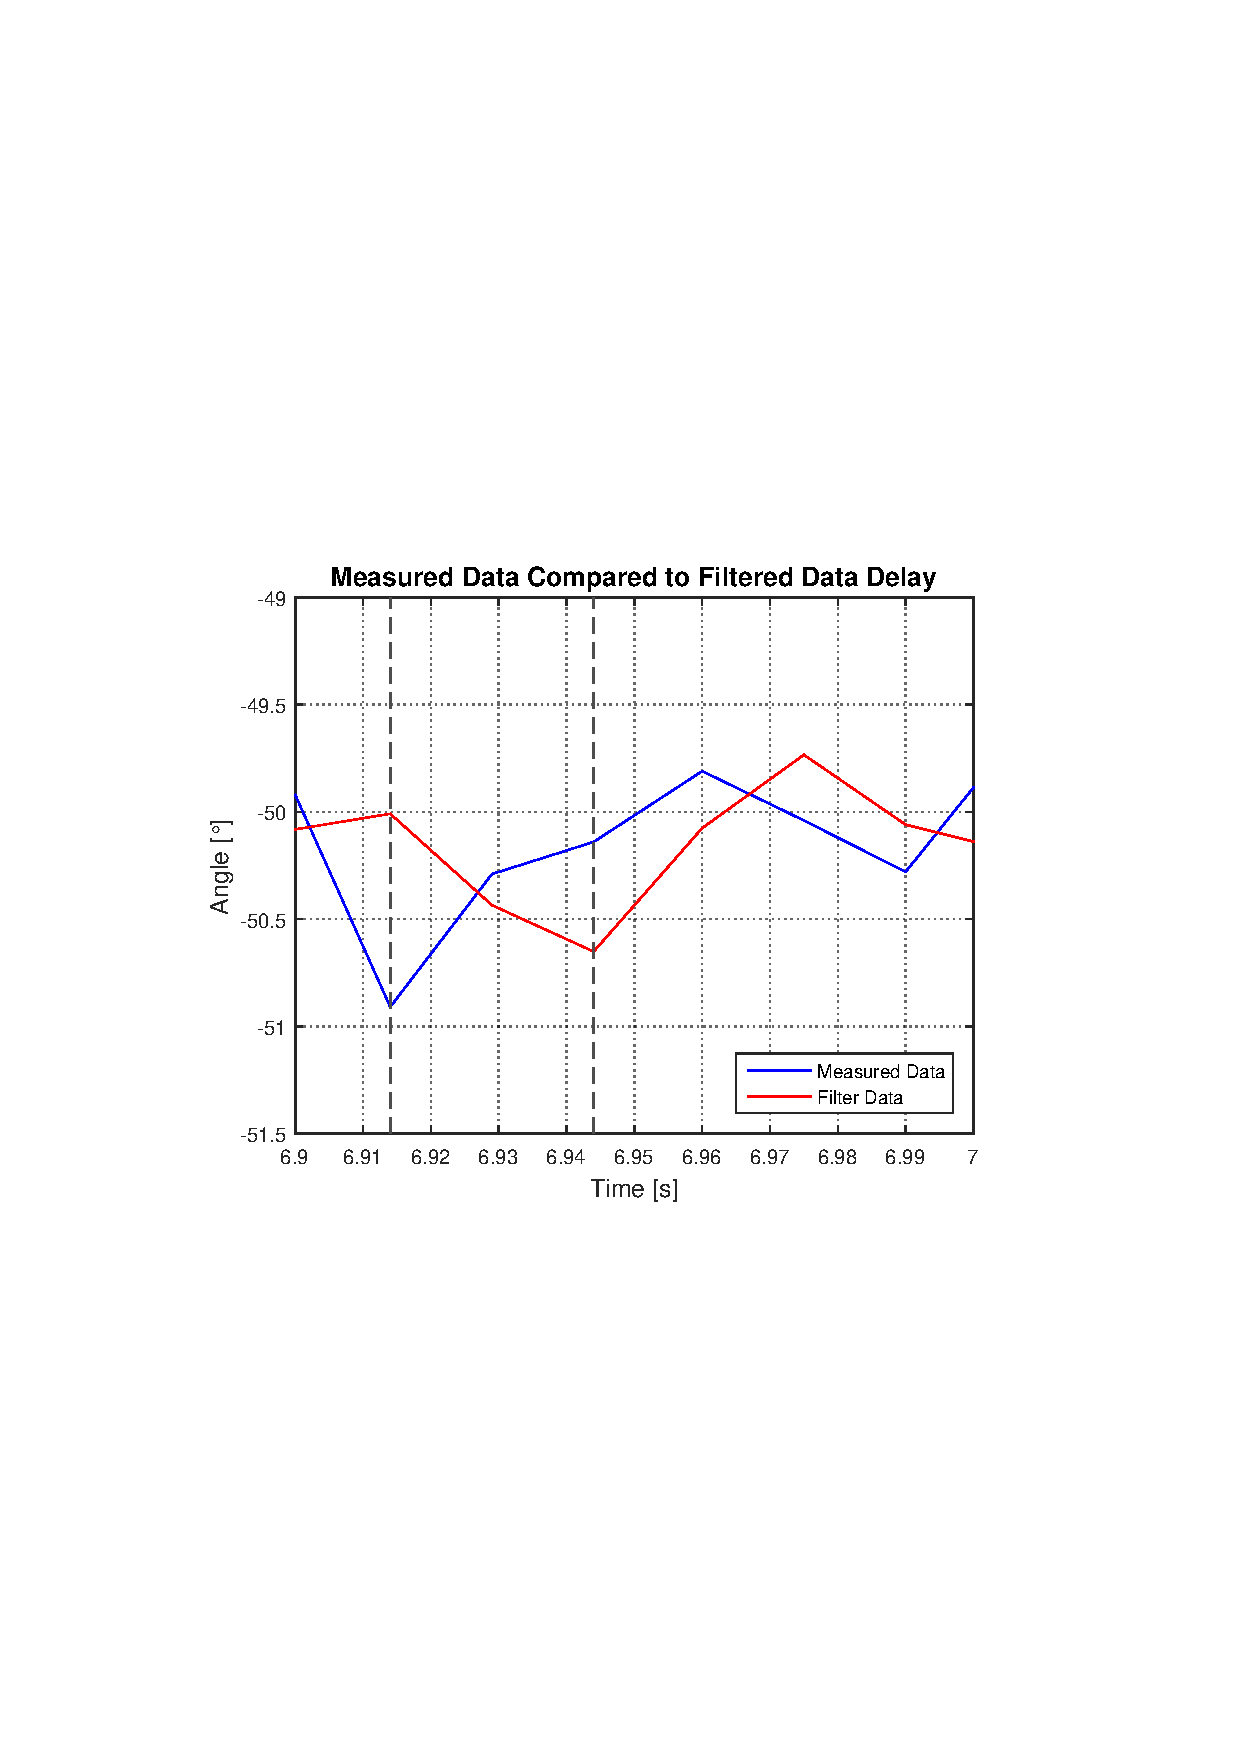
\includegraphics[scale = .5]{Pictures/FinalimplementationFilterDelay.pdf}
  \end{figure}
\end{frame}

%%%%%%%%%%%%%%%%